\documentclass[12pt,a4paper]{article}
\usepackage[polish]{babel}
\usepackage[utf8]{inputenc}
\usepackage[T1]{fontenc}

% dodatkowe rodzaje punktorów
%\usepackage{enumerate}

%symbole matematyczne
\usepackage{amsmath}

%układ strony
\usepackage{fancyhdr}

%zaawansowane marginesy
%\usepackage{a4wide}

%pobieranie obrazków z pdf
%\usepackage{pdfpages} 

\usepackage[pdftex]{graphicx}
\usepackage{multirow}

%listningi
\usepackage{listings}
\lstloadlanguages{TeX}

%konfiguracja MATLABowego listningu
\usepackage{color} %red, green, blue, yellow, cyan, magenta, black, white
\definecolor{mygreen}{RGB}{28,172,0} % color values Red, Green, Blue
\definecolor{mylilas}{RGB}{170,55,241}
\lstset{language=Matlab,%
    %basicstyle=\color{red},
    breaklines=true,%
    morekeywords={matlab2tikz},
    keywordstyle=\color{blue},%
    morekeywords=[2]{1}, keywordstyle=[2]{\color{black}},
    identifierstyle=\color{black},%
    stringstyle=\color{mylilas},
    commentstyle=\color{mygreen},%
    showstringspaces=false,%without this there will be a symbol in the places where there is a space
    numbers=left,%
    numberstyle={\tiny \color{black}},% size of the numbers
    numbersep=9pt, % this defines how far the numbers are from the text
    emph=[1]{for,end,break},emphstyle=[1]\color{blue}, %some words to emphasise
    %emph=[2]{word1,word2}, emphstyle=[2]{style},    
}

%polskie znaki
\lstset{
  literate={ą}{{\k{a}}}1
           {ć}{{\'c}}1
           {ę}{{\k{e}}}1
           {ó}{{\'o}}1
           {ń}{{\'n}}1
           {ł}{{\l{}}}1
           {ś}{{\'s}}1
           {ź}{{\'z}}1
           {ż}{{\.z}}1
           {Ą}{{\k{A}}}1
           {Ć}{{\'C}}1
           {Ę}{{\k{E}}}1
           {Ó}{{\'O}}1
           {Ń}{{\'N}}1
           {Ł}{{\L{}}}1
           {Ś}{{\'S}}1
           {Ź}{{\'Z}}1
           {Ż}{{\.Z}}1
}

%włączenie barwnych hiperłączy
%\usepackage[colorlinks=true,urlcolor=blue,linkcolor=red,citecolor=green]{hyperref}
\usepackage[colorlinks=true,urlcolor=black,linkcolor=black,citecolor=black]{hyperref}

%marginesy
\usepackage{geometry}
\newgeometry{tmargin=2.5cm, bmargin=2.5cm, lmargin=2.5cm, rmargin=2.5cm}

%wykresy z matlaba
\usepackage{pgfplots}

%kropki przy numeracji
%\renewcommand\thesection{\arabic{section}.}
%\renewcommand\thesubsection{\thesection\arabic{subsection}.}

%dane pliku
\author
{Jakub Porębski,$^{1,2,a\ast}$ Żaneta Błaszczuk,$^{1,b}$ Jakub Szczepankiewicz$^{1, c}$\\
\\
\normalsize{$^{1}$Wydział Elektrotechniki, Automatyki, Informatyki i Inżynierii Biomedycznej,}\\
\normalsize{Akademia Górniczo-Hutnicza, Al. Mickiewicza 30}\\
\normalsize{$^{2}$Wydział Inżynierii Materiałowej i Ceramiki,}\\ \normalsize{Akademia Górniczo-Hutnicza, Al. Mickiewicza 30}\\
\\
\normalsize{$^a$amalgamat321@gmail.com, $^b$zaneta.blaszczuk@gmail.com ,}\\
\normalsize{$^c$ szczepankiewiczjakub7@gmail.com}
}
\title{System pomiarowy do oceny jakości powietrza \\i warunków otoczenia w domu \\ \Huge{$\mu$ KLIMAT}}	
%\title{Stacja pomiarowo-badawcza \\oceniająca jakość domowego ekosystemu \\ \Huge{$\mu$ KLIMAT}}
\date{}

%nagłówek strony
\pagestyle{fancy}
\fancyhead[R]{Ż. Błaszczuk, J. Porębski, J. Szczepankiewicz}
\fancyhead[L]{$\mu$ KLIMAT} 		
\fancyfoot[C]{\thepage}

\begin{document}
%\input{./titlepage.tex}
\maketitle
\begin{figure}[!h]
\centering
	
\includegraphics[height =40mm]{agh.jpg}\\[1cm]
	
\includegraphics[height =40mm]{logo.jpg}
\end{figure}
\newpage


\section{Szczegóły realizacji}
\subsection{O projekcie}
Dom jest najważniejszym środowiskiem, w jakim żyjemy. Dbamy o niego i staramy się, by panowała w nim „zdrowa” atmosfera. Nasze urządzenie pomaga utrzymać odpowiedni mikroklimat w mieszkaniu, tak aby zatrzymać rozwój mikroorganizmów i zapewnić jak najmniejszy poziom zanieczyszczeń. Zbudowana przez nas stacja pomiarowa pozwala na pomiar temperatury, ciśnienia, wilgotności, oświetlenia oraz stężenia dwutlenku węgla. Dodatkowo urządzenie może służyć jako alkomat, który mierzy stężenie etanolu w wydychanym powietrzu. Dzięki zastosowaniu czujników elektrochemicznych urządzenie jest bardzo wrażliwe na inne szkodliwe gazy takie jak tlenek węgla, metan, a nawet dym. Pozwala to na wykrywanie sytuacji alarmowych i czyni z urządzenia kompaktowy wykrywacz dymu, zaczadzenia oraz wycieków gazu.

Naszym celem jest wykształcenie zdrowych zachowań u mieszkańców, dlatego \textit{$\mu$KLIMAT} nie posiada całkowitej kontroli nad ekosystemem mieszkania. Urządzenie wyświetla zebrane dane na wyświetlaczu LCD oraz wysyła je do aplikacji mobilnej poprzez sieć WiFi. Aplikacja ostrzega przed potencjalnym zagrożeniem oraz proponuje odpowiednie rozwiązanie np: gdy wilgotność w pomieszczeniu przekracza 60\% aplikacja zaleca otwarcie okna i przewietrzenie pokoju. Co więcej aplikacja informuje, że podwyższona wilgotność może wywoływać bóle głowy i uczucie duszności. 

Dla zaawansowanych użytkowników jest również przygotowany system akwizycji danych, który pozwala na prezentację zmienności na wykresach.

\subsection{Rozwiązania wykorzystane w projekcie}
\subsubsection{Mikroprocesor}
Stacja badawcza została zbudowana w oparciu o zestaw ewaluacyjny \textit{FRDM KL25Z} firmy Freescale z mikroprocesorem ARM\textregistered Cortex$^{\textsc{TM}}$-M0. Wybrano ten zestaw ze względu na dużą liczbę wejść analogowych, 3 porty szeregowe i 3 interfejsy ISP.
\subsubsection{Sensory}
W celu zapewnienia jak największego przekroju badanych parametrów zastosowano 5 różnych czujników:
\begin{enumerate}
	\item[1)] Czujniki elektrochemiczne\\
	Czujniki te wykorzystują reakcję chemiczną zachodzącą w podwyższonej temperaturze na elektrodzie detekcyjnej (zbudowanej z $SnO2$), aby wywołać różnicę potencjałów między elektrodą zliczającą ($Au$), a referencyjną ($Pt$). Zaletą takich czujników jest ich łatwa do opisania charakterystyka oraz wrażliwość na rzadko występujące, lecz bardzo szkodliwe dla zdrowia gazy. 

	Wadą jest konieczność jednorazowej kalibracji każdego czujnika. Dobór parametrów czujników został zrealizowany w programie MATLAB z wykorzystaniem czujnika referencyjnego.

\newpage

	\begin{enumerate}
		\item[a)] Czujnik jakości powietrza - MQ135 \\
		Czujnik MQ135 jest najbardziej wrażliwy na stężenie dwutlenku węgla, które może mierzyć w zakresie 200-2000 ppm. Ponadto czujnik ten może posłużyć jako wyrywacz dymu i zaczadzenia.
		
\begin{figure}[!h]
	\centering
	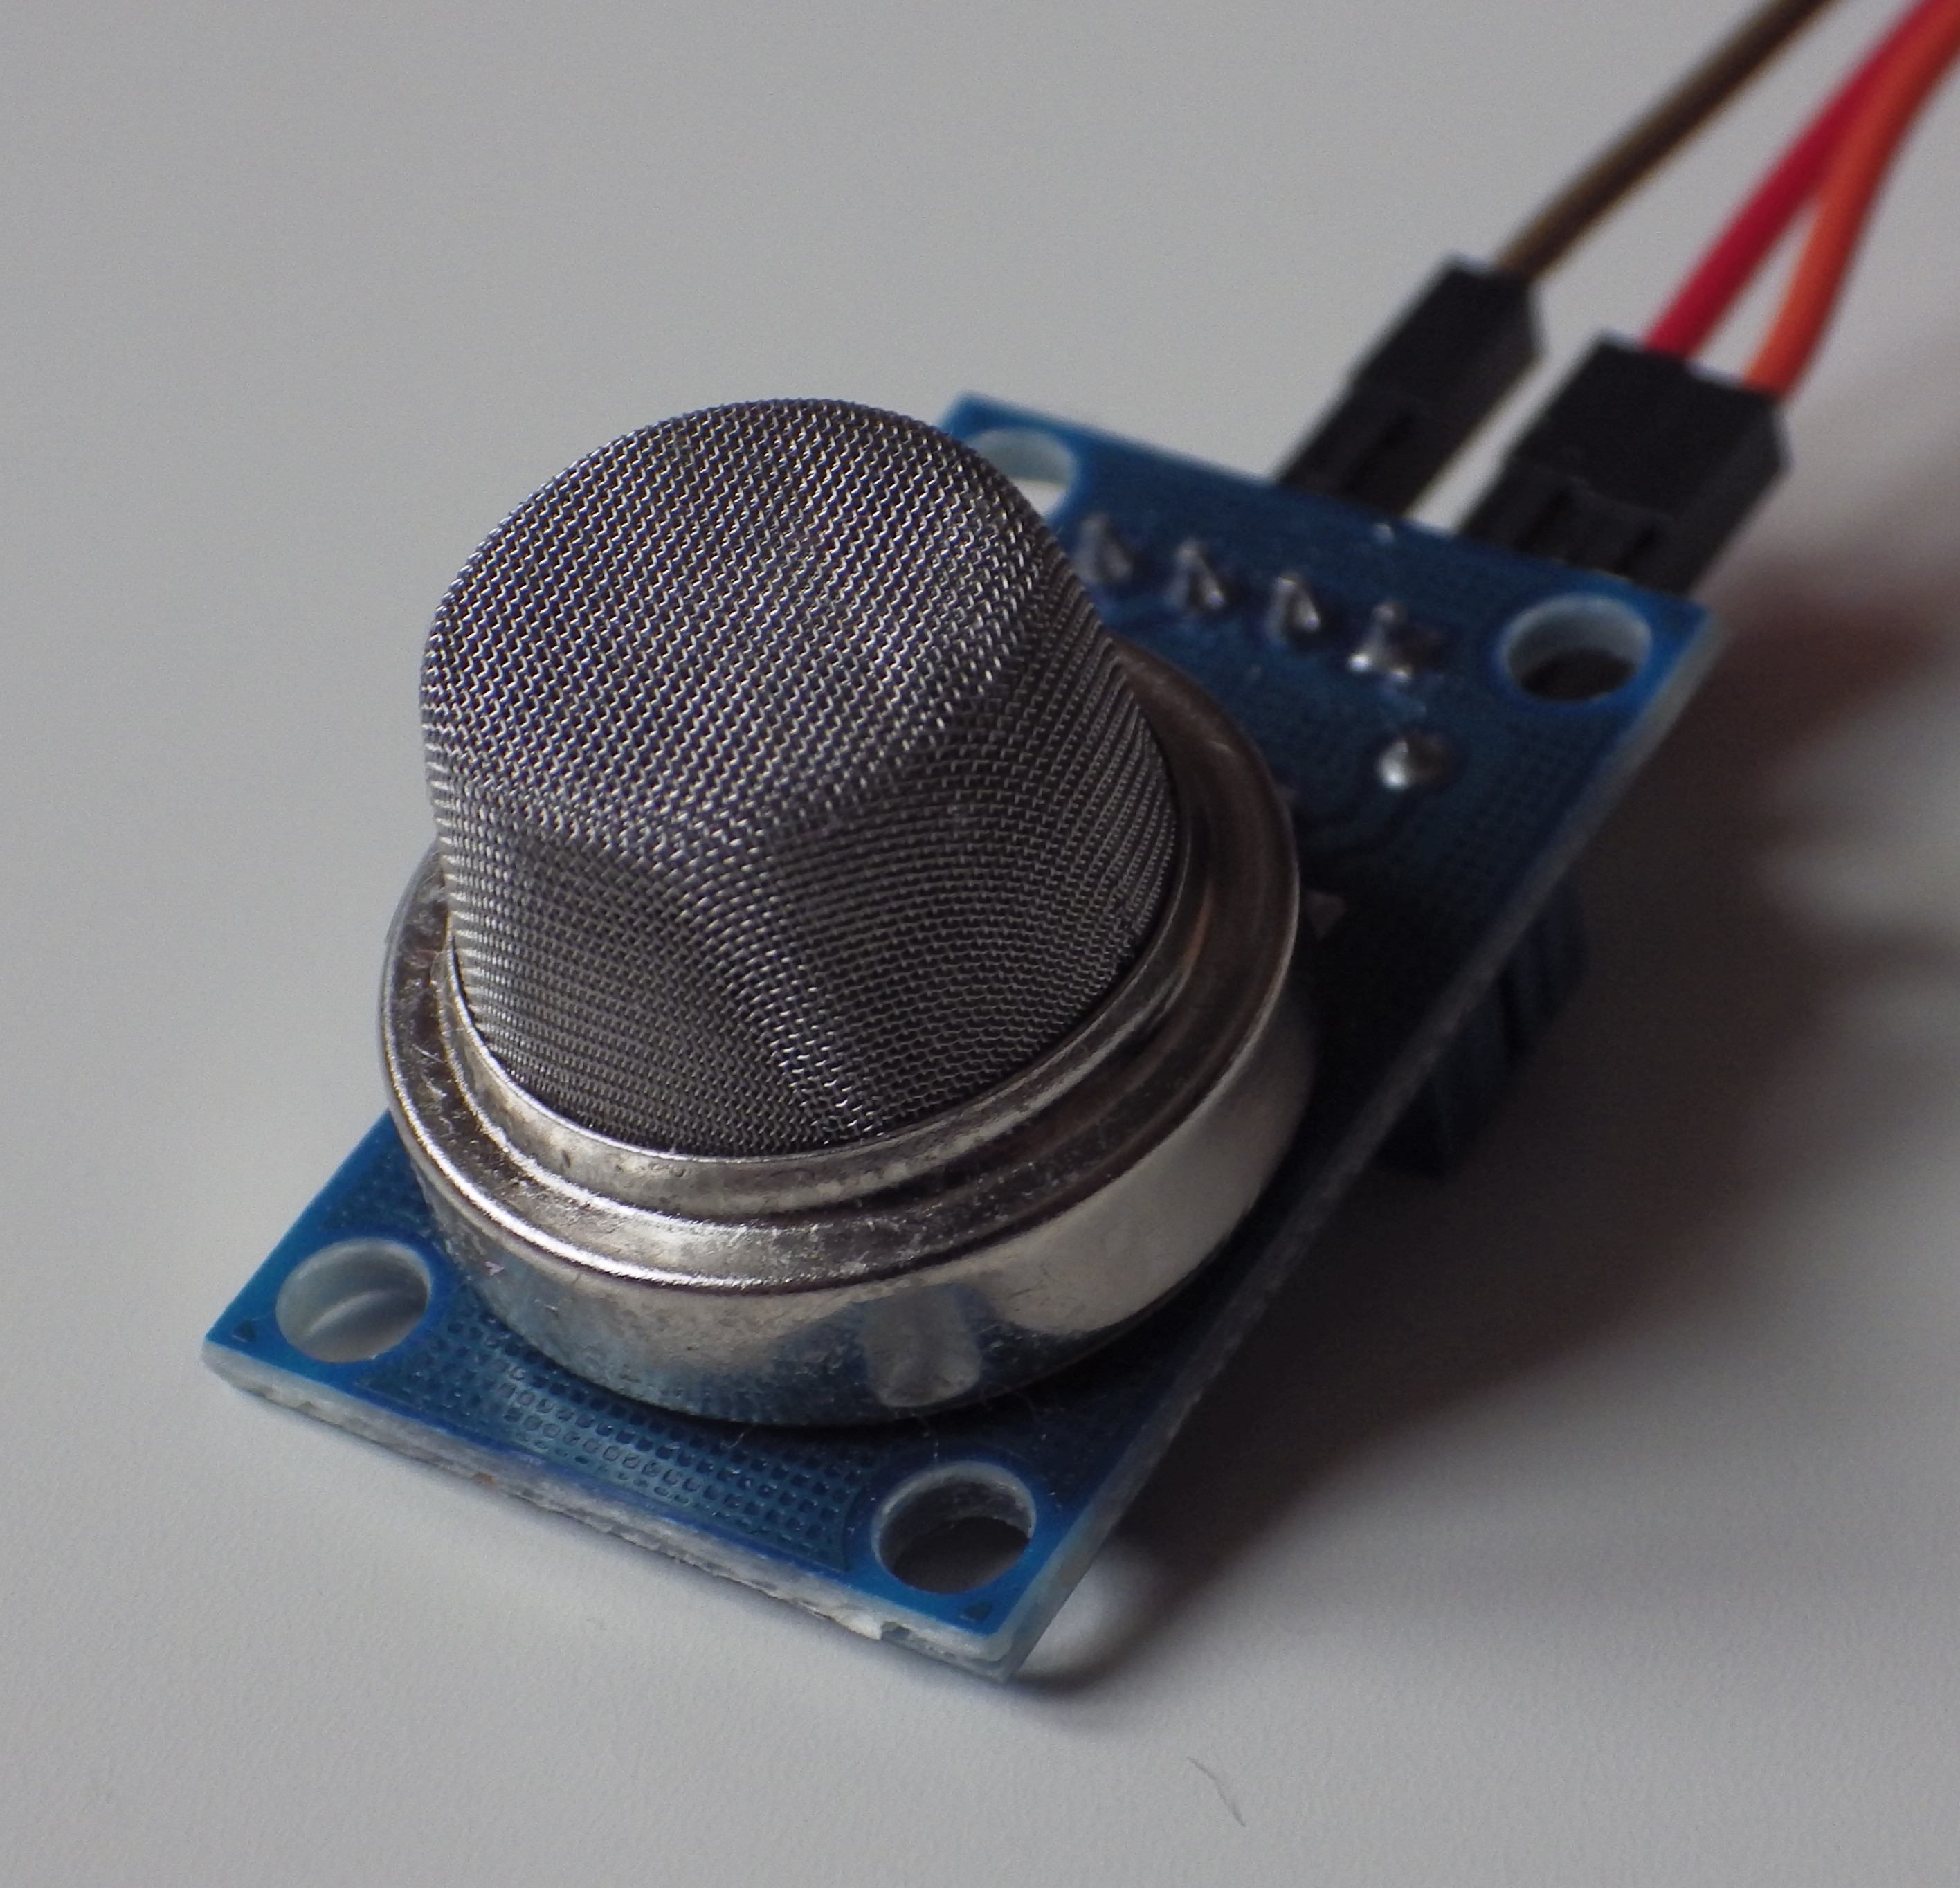
\includegraphics[height =60mm]{MQ135.jpg}
	\label{MQ135}
	\caption{Czujnik jakości powietrza MQ135 służy do pomiaru stężenia $CO_2$ oraz poziomów alarmowych czadu i dymu}
\end{figure}

		\item[b)] Czujnik alkoholu - MQ3 \\	
		Czujnik MQ3 poza wykrywaniem etanolu jest również wrażliwy na metan, dzięki czemu wykryje wszelkiego rodzaju wycieki gazu.
		
\begin{figure}[!h]	
\centering
	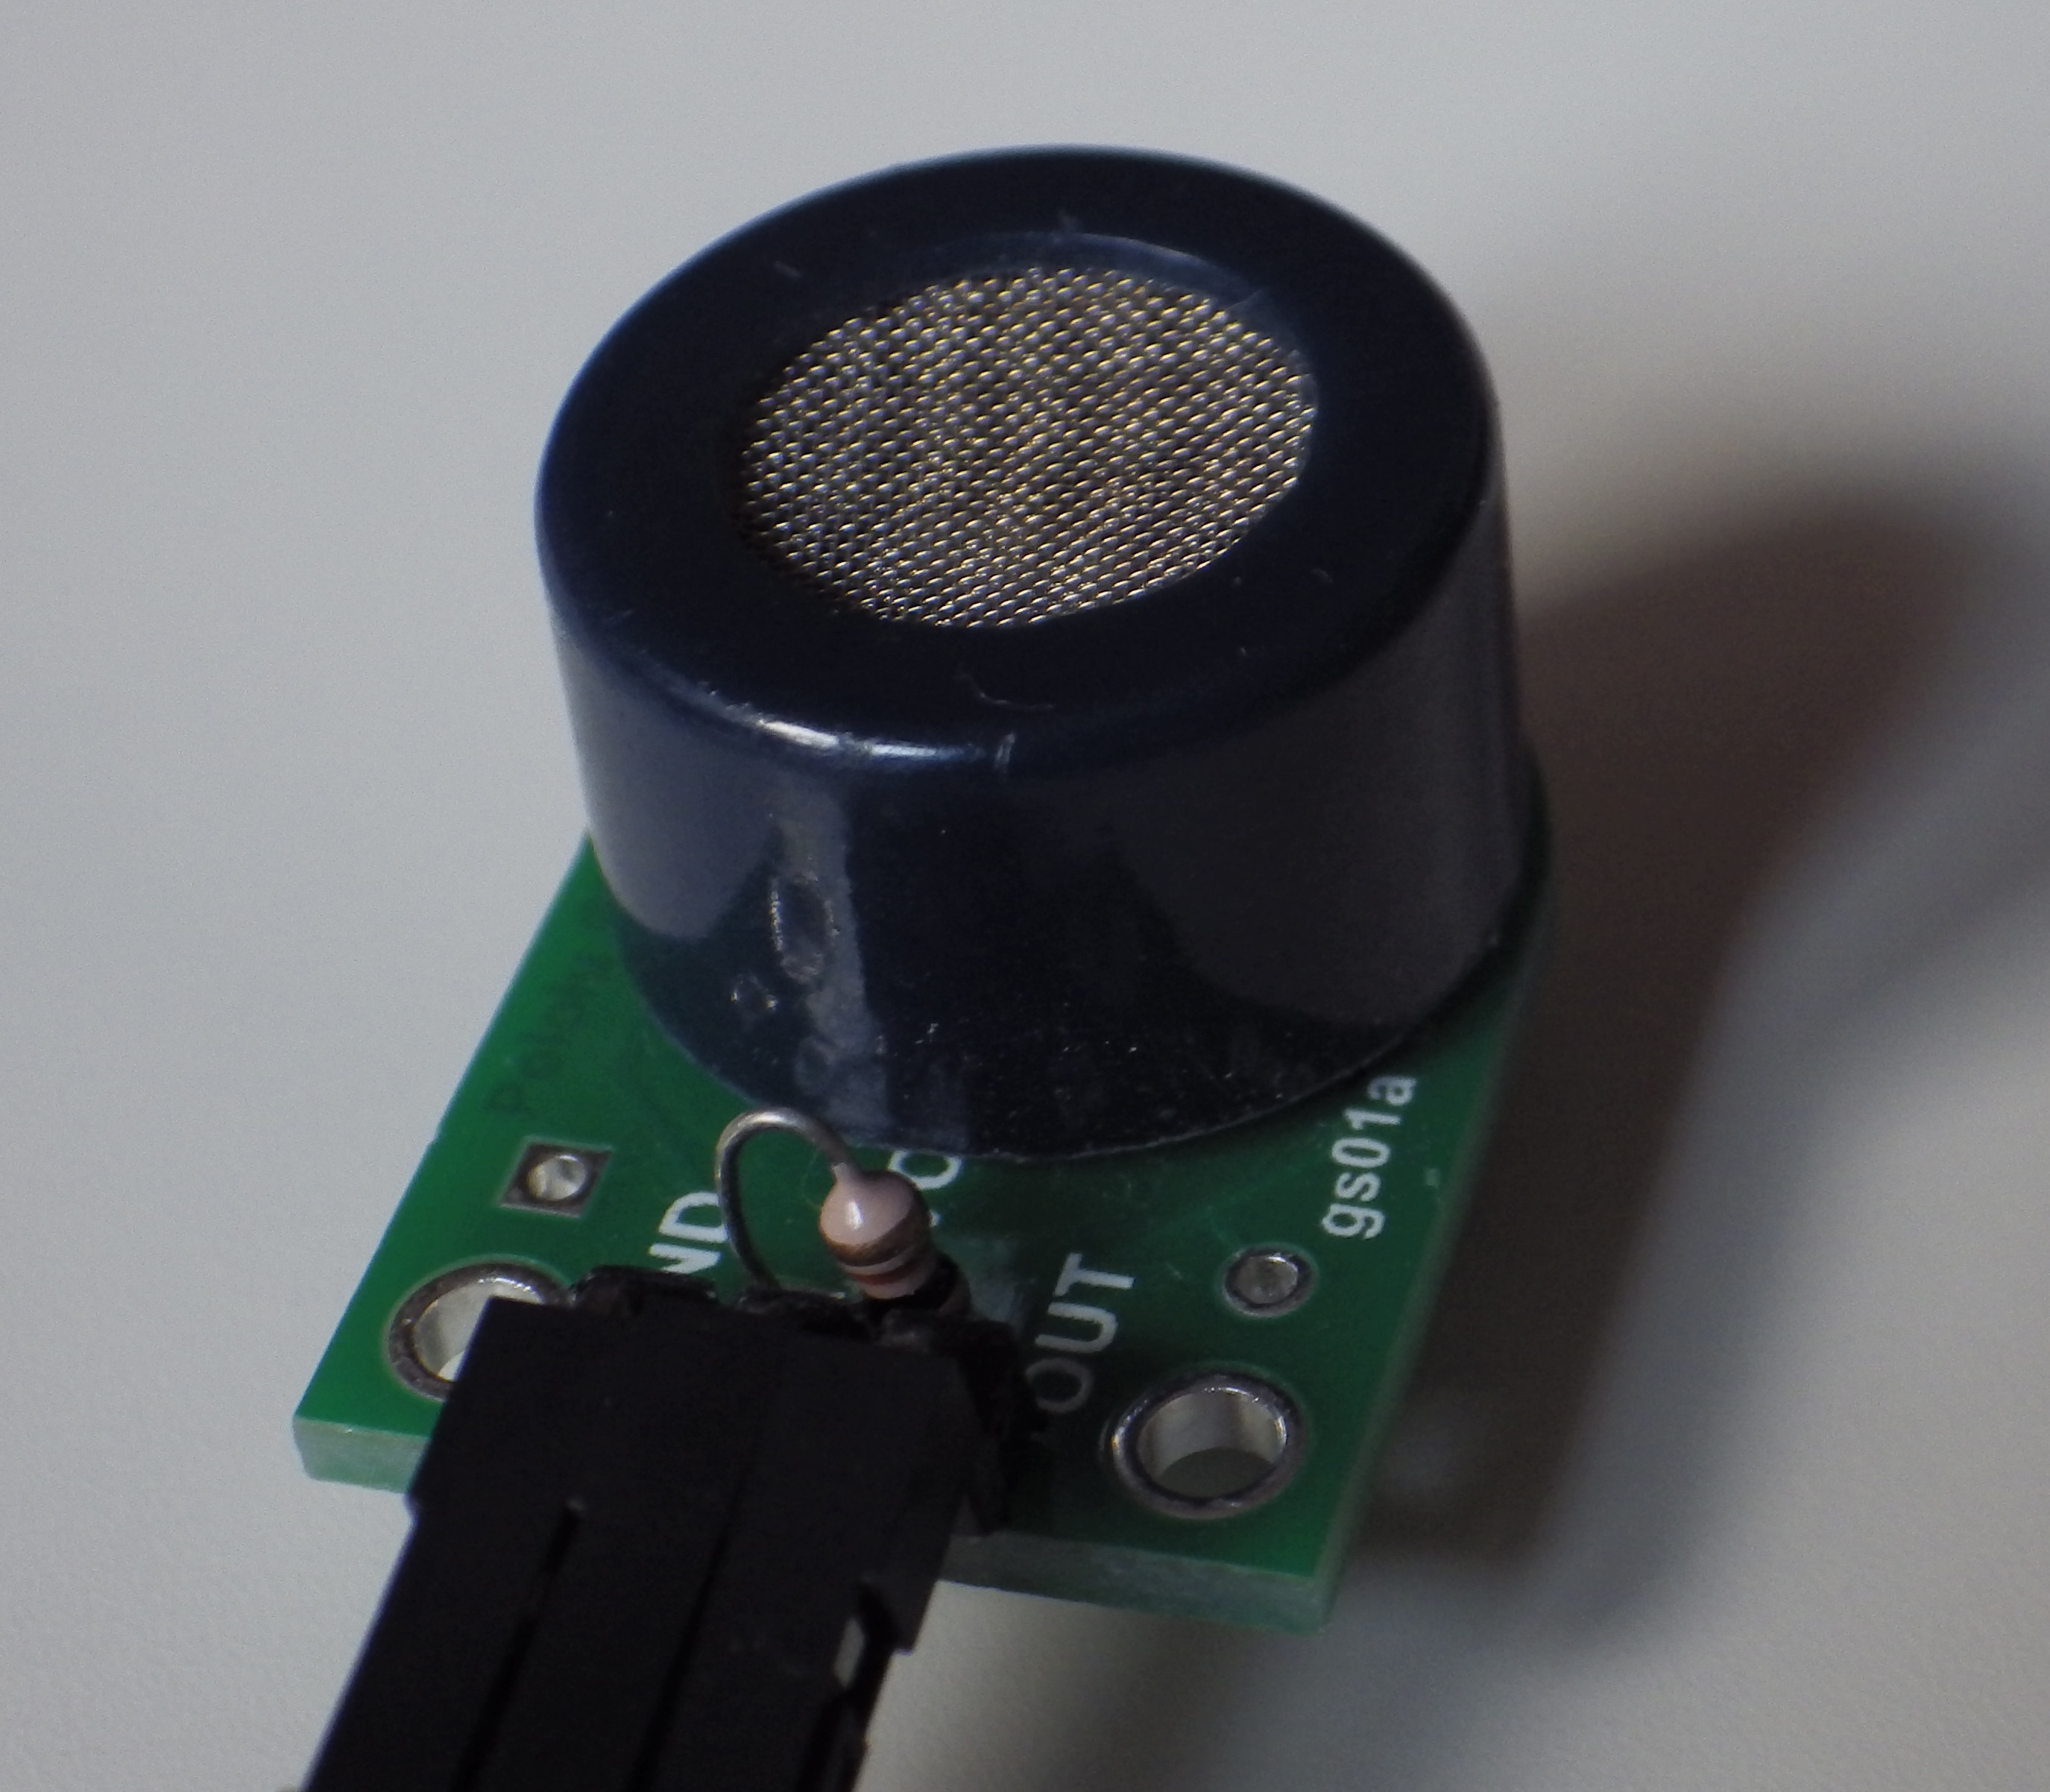
\includegraphics[height =60mm]{MQ3.jpg}
	\label{MQ3}
	\caption{Czujnik alkoholu i wycieków gazu -- MQ3}
\end{figure}		
	
	\end{enumerate}	
	
\newpage
	
	\item[2)]Czujnik temperatury i ciśnienia - BMP180\\
	Ten czujnik firmy Bosch został wyprodukowany w technologii MEMS i pozwala na bardzo dokładny pomiar temperatury i ciśnienia z dużą dokładnością.

\begin{figure}[!h]	
\centering
	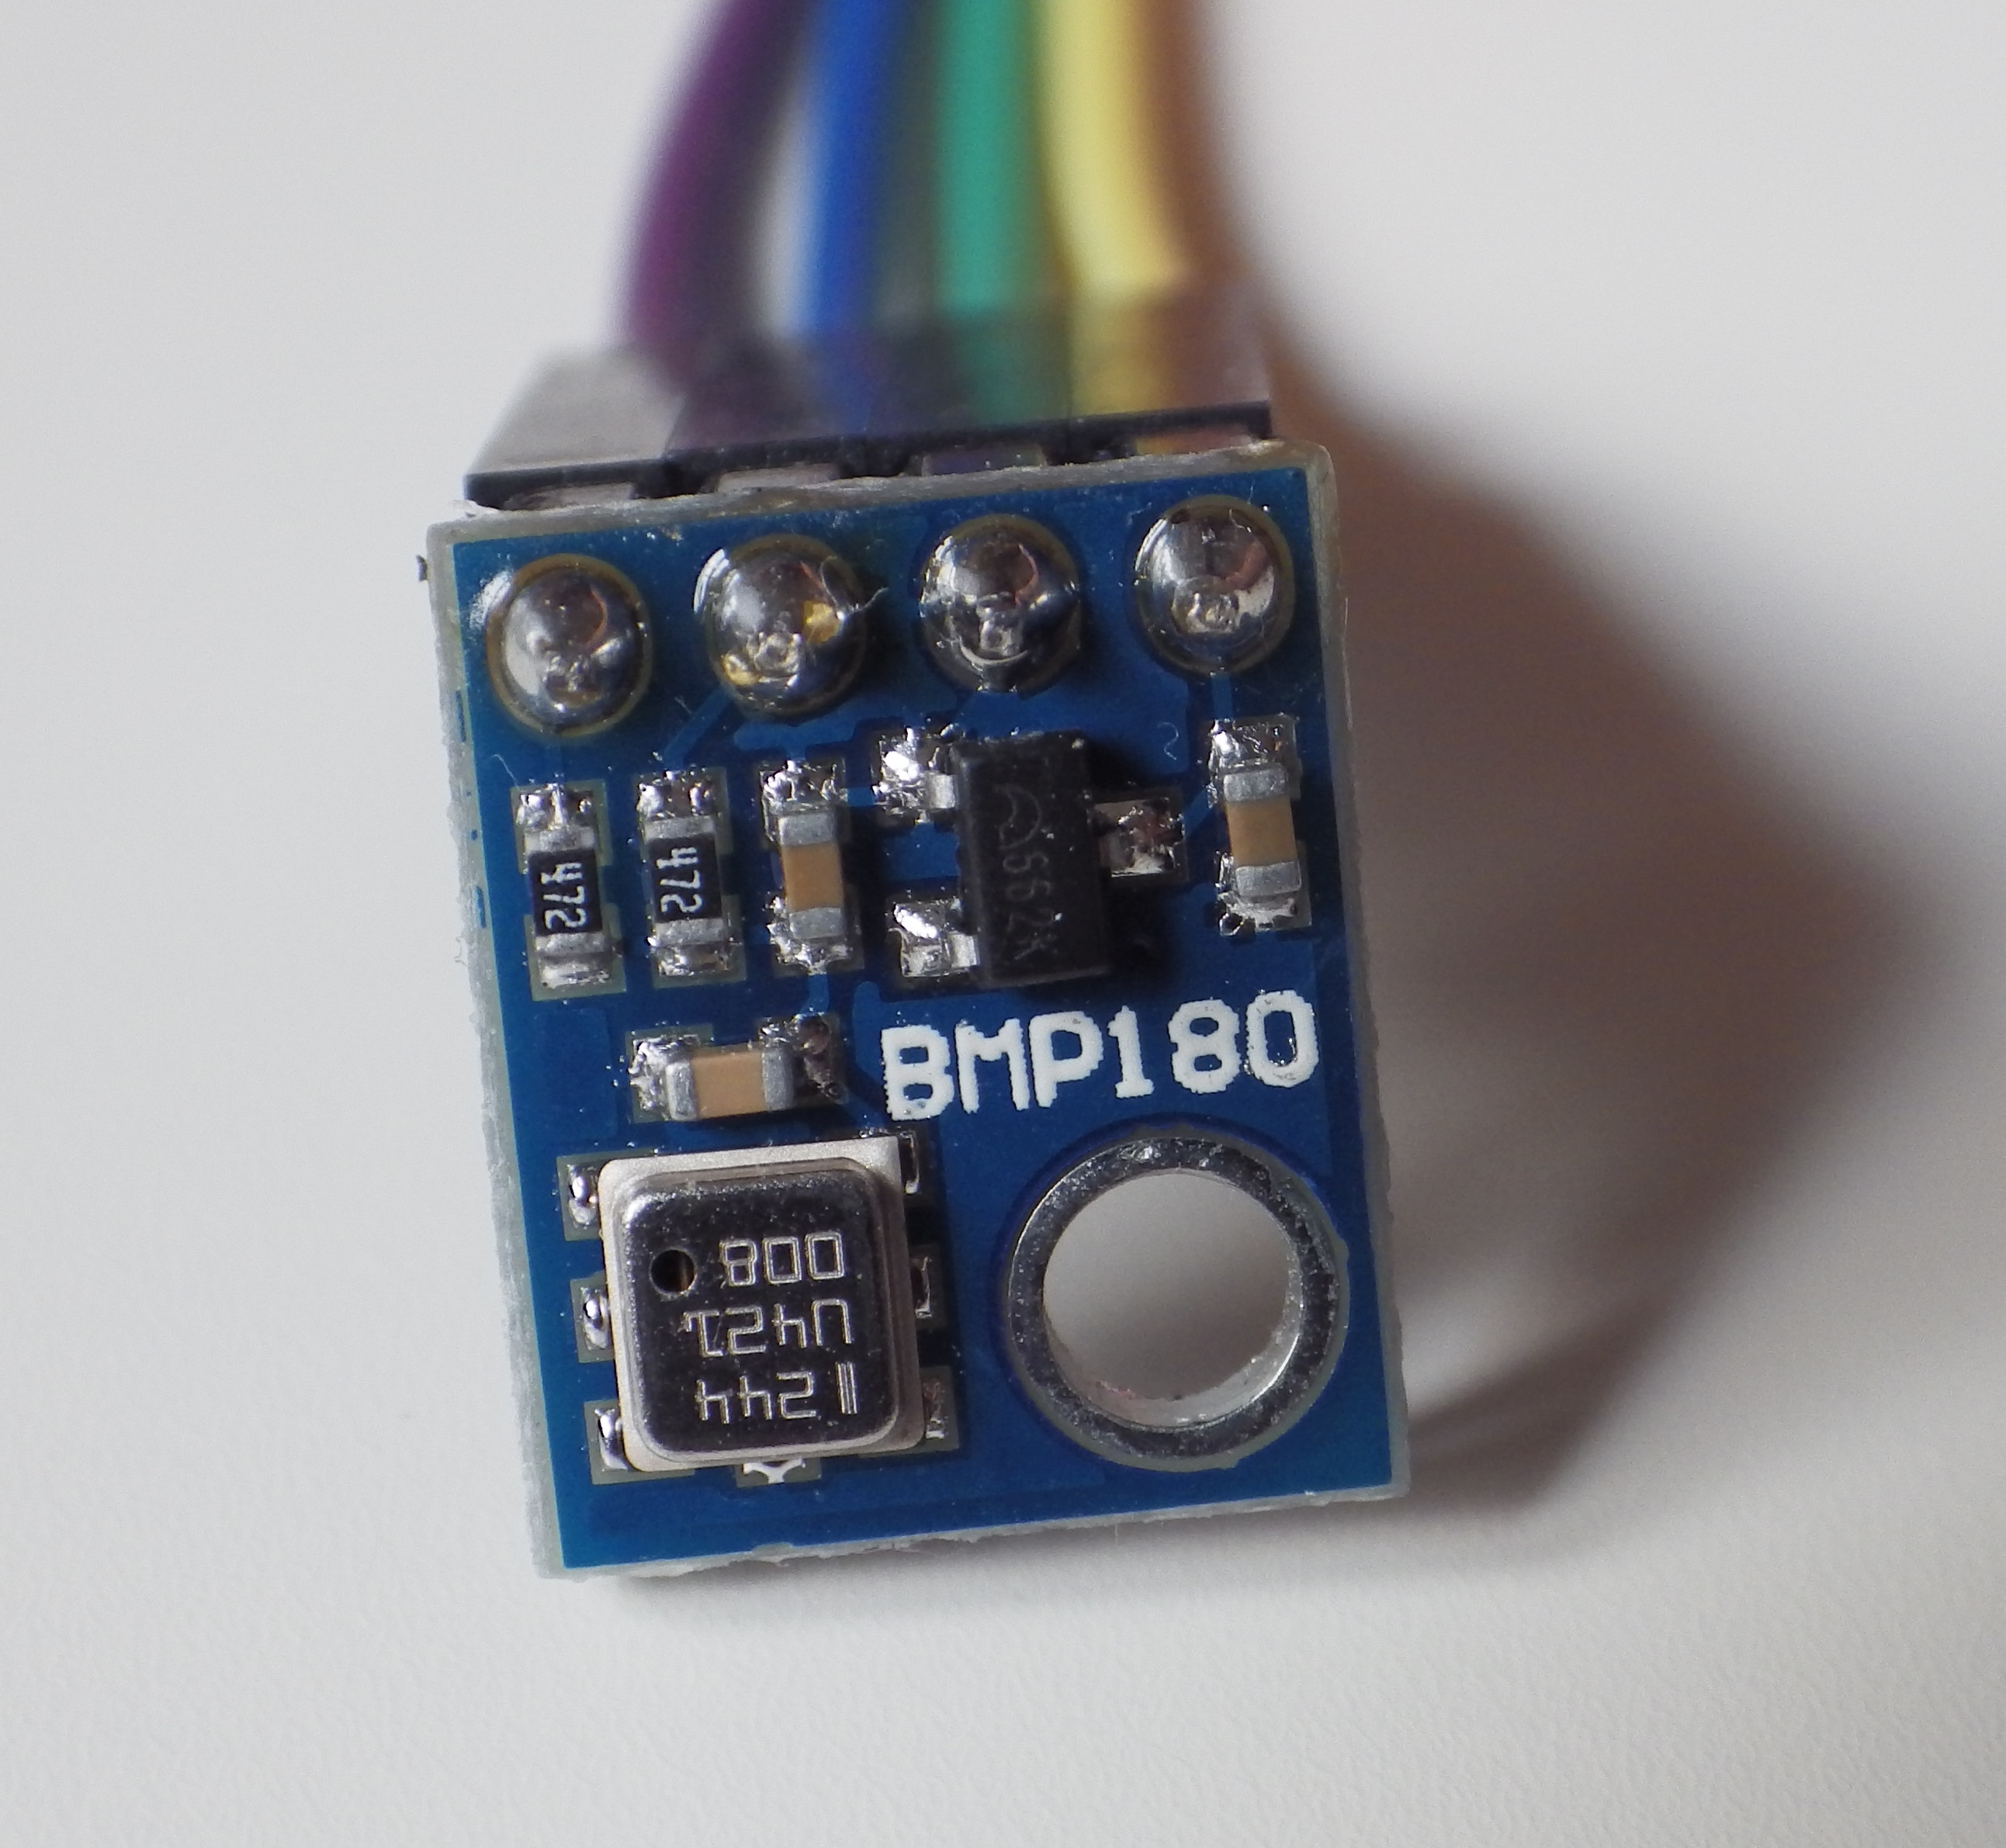
\includegraphics[height =50mm]{BMP180.jpg}
	\label{BMP180}
	\caption{Czujnik temperatury i ciśnienia -- BMP180}
\end{figure}	
	
	\item[3)]Fotorezystor\\
	W celu pomiaru poziomu oświetlenia wykorzystano fotorezystor $5-10k\Omega$.

\begin{figure}[!h]	
\centering
	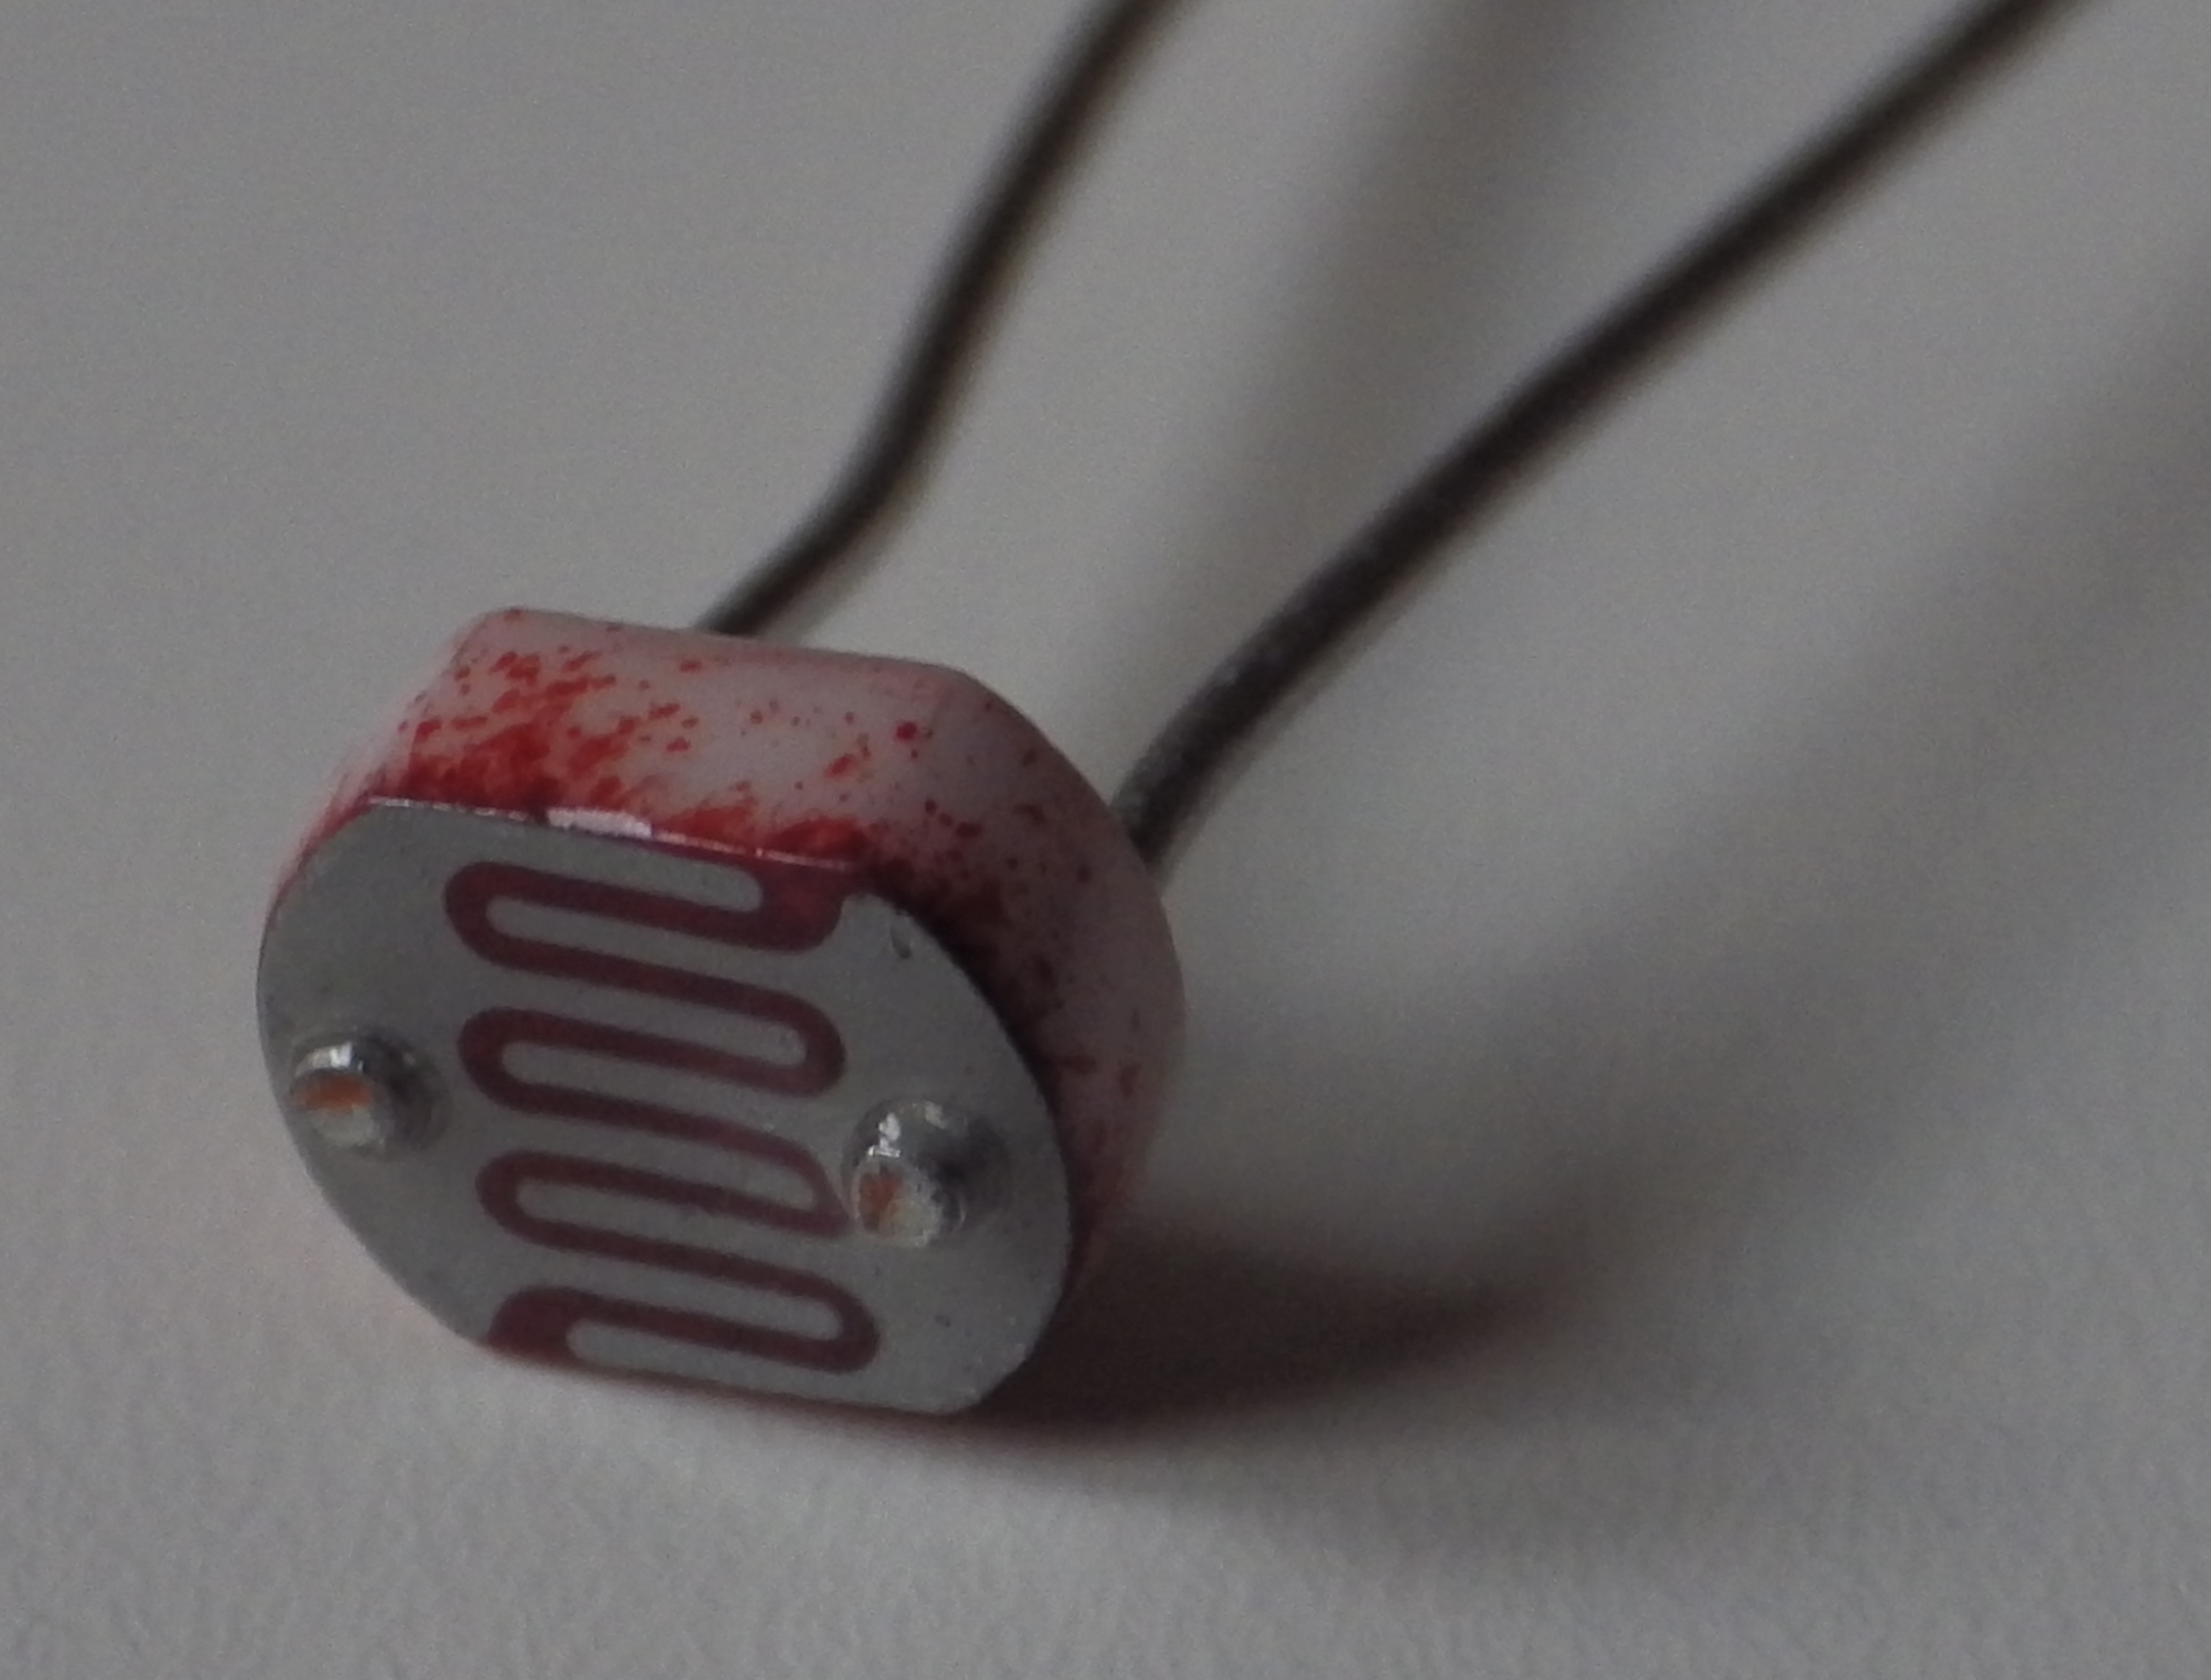
\includegraphics[height =50mm]{fotorezystor.jpg}
	\label{fotorezystor}
	\caption{Fotorezystor $5-10k\Omega$}
\end{figure}	
	
	\item[4)]Czujnik wilgotności -- DHT11\\
	Jest to czujnik pojemnościowy, który pozwala na pomiar wilgotności względnej w zakresie od 30\% do 80\%.

\begin{figure}[!h]	
\centering
	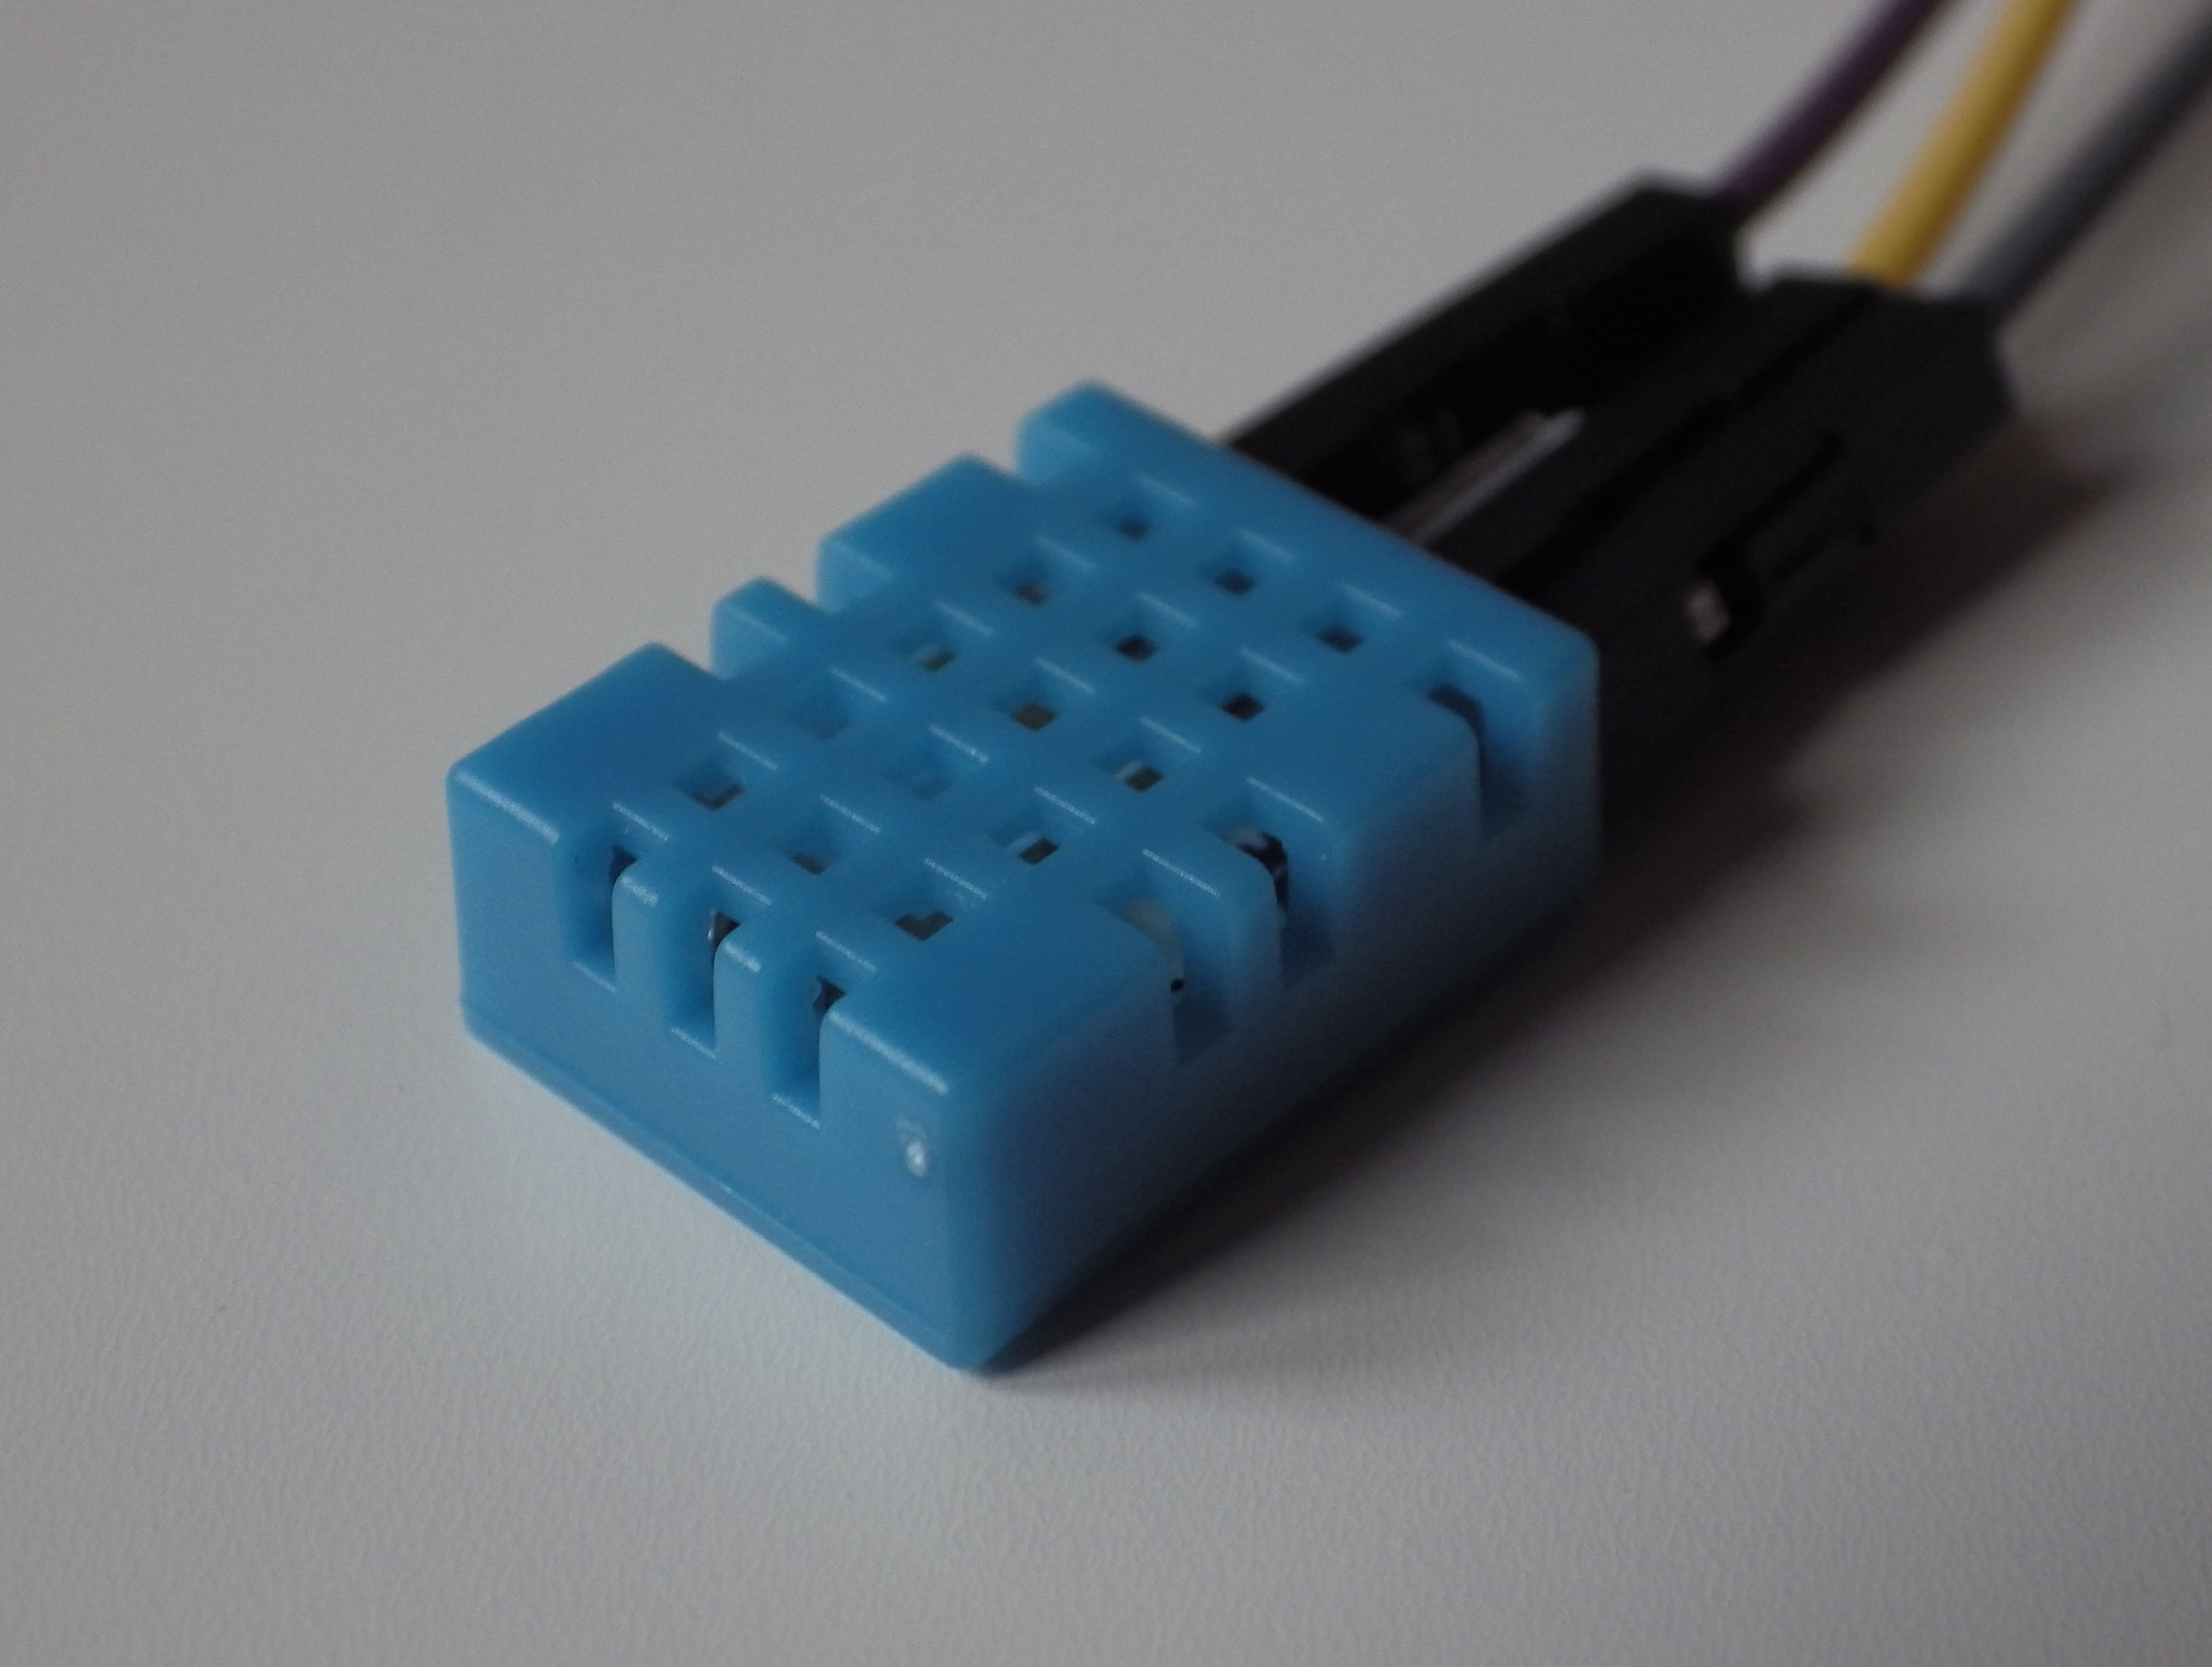
\includegraphics[height =50mm]{DHT11.jpg}
	\label{DHT11}
	\caption{Pojemnościowy czujnik wilgotności -- DHT11}
\end{figure}		
	
\end{enumerate}
\subsubsection{Komunikacja}
Dane odczytywane z czujników są wyświetlane na ekranie LCD oraz wysyłane poprzez sieć WiFi do aplikacji mobilnej.
% Typ ekranu LCD to: JHD 204A
\begin{figure}[!h]	
\centering
	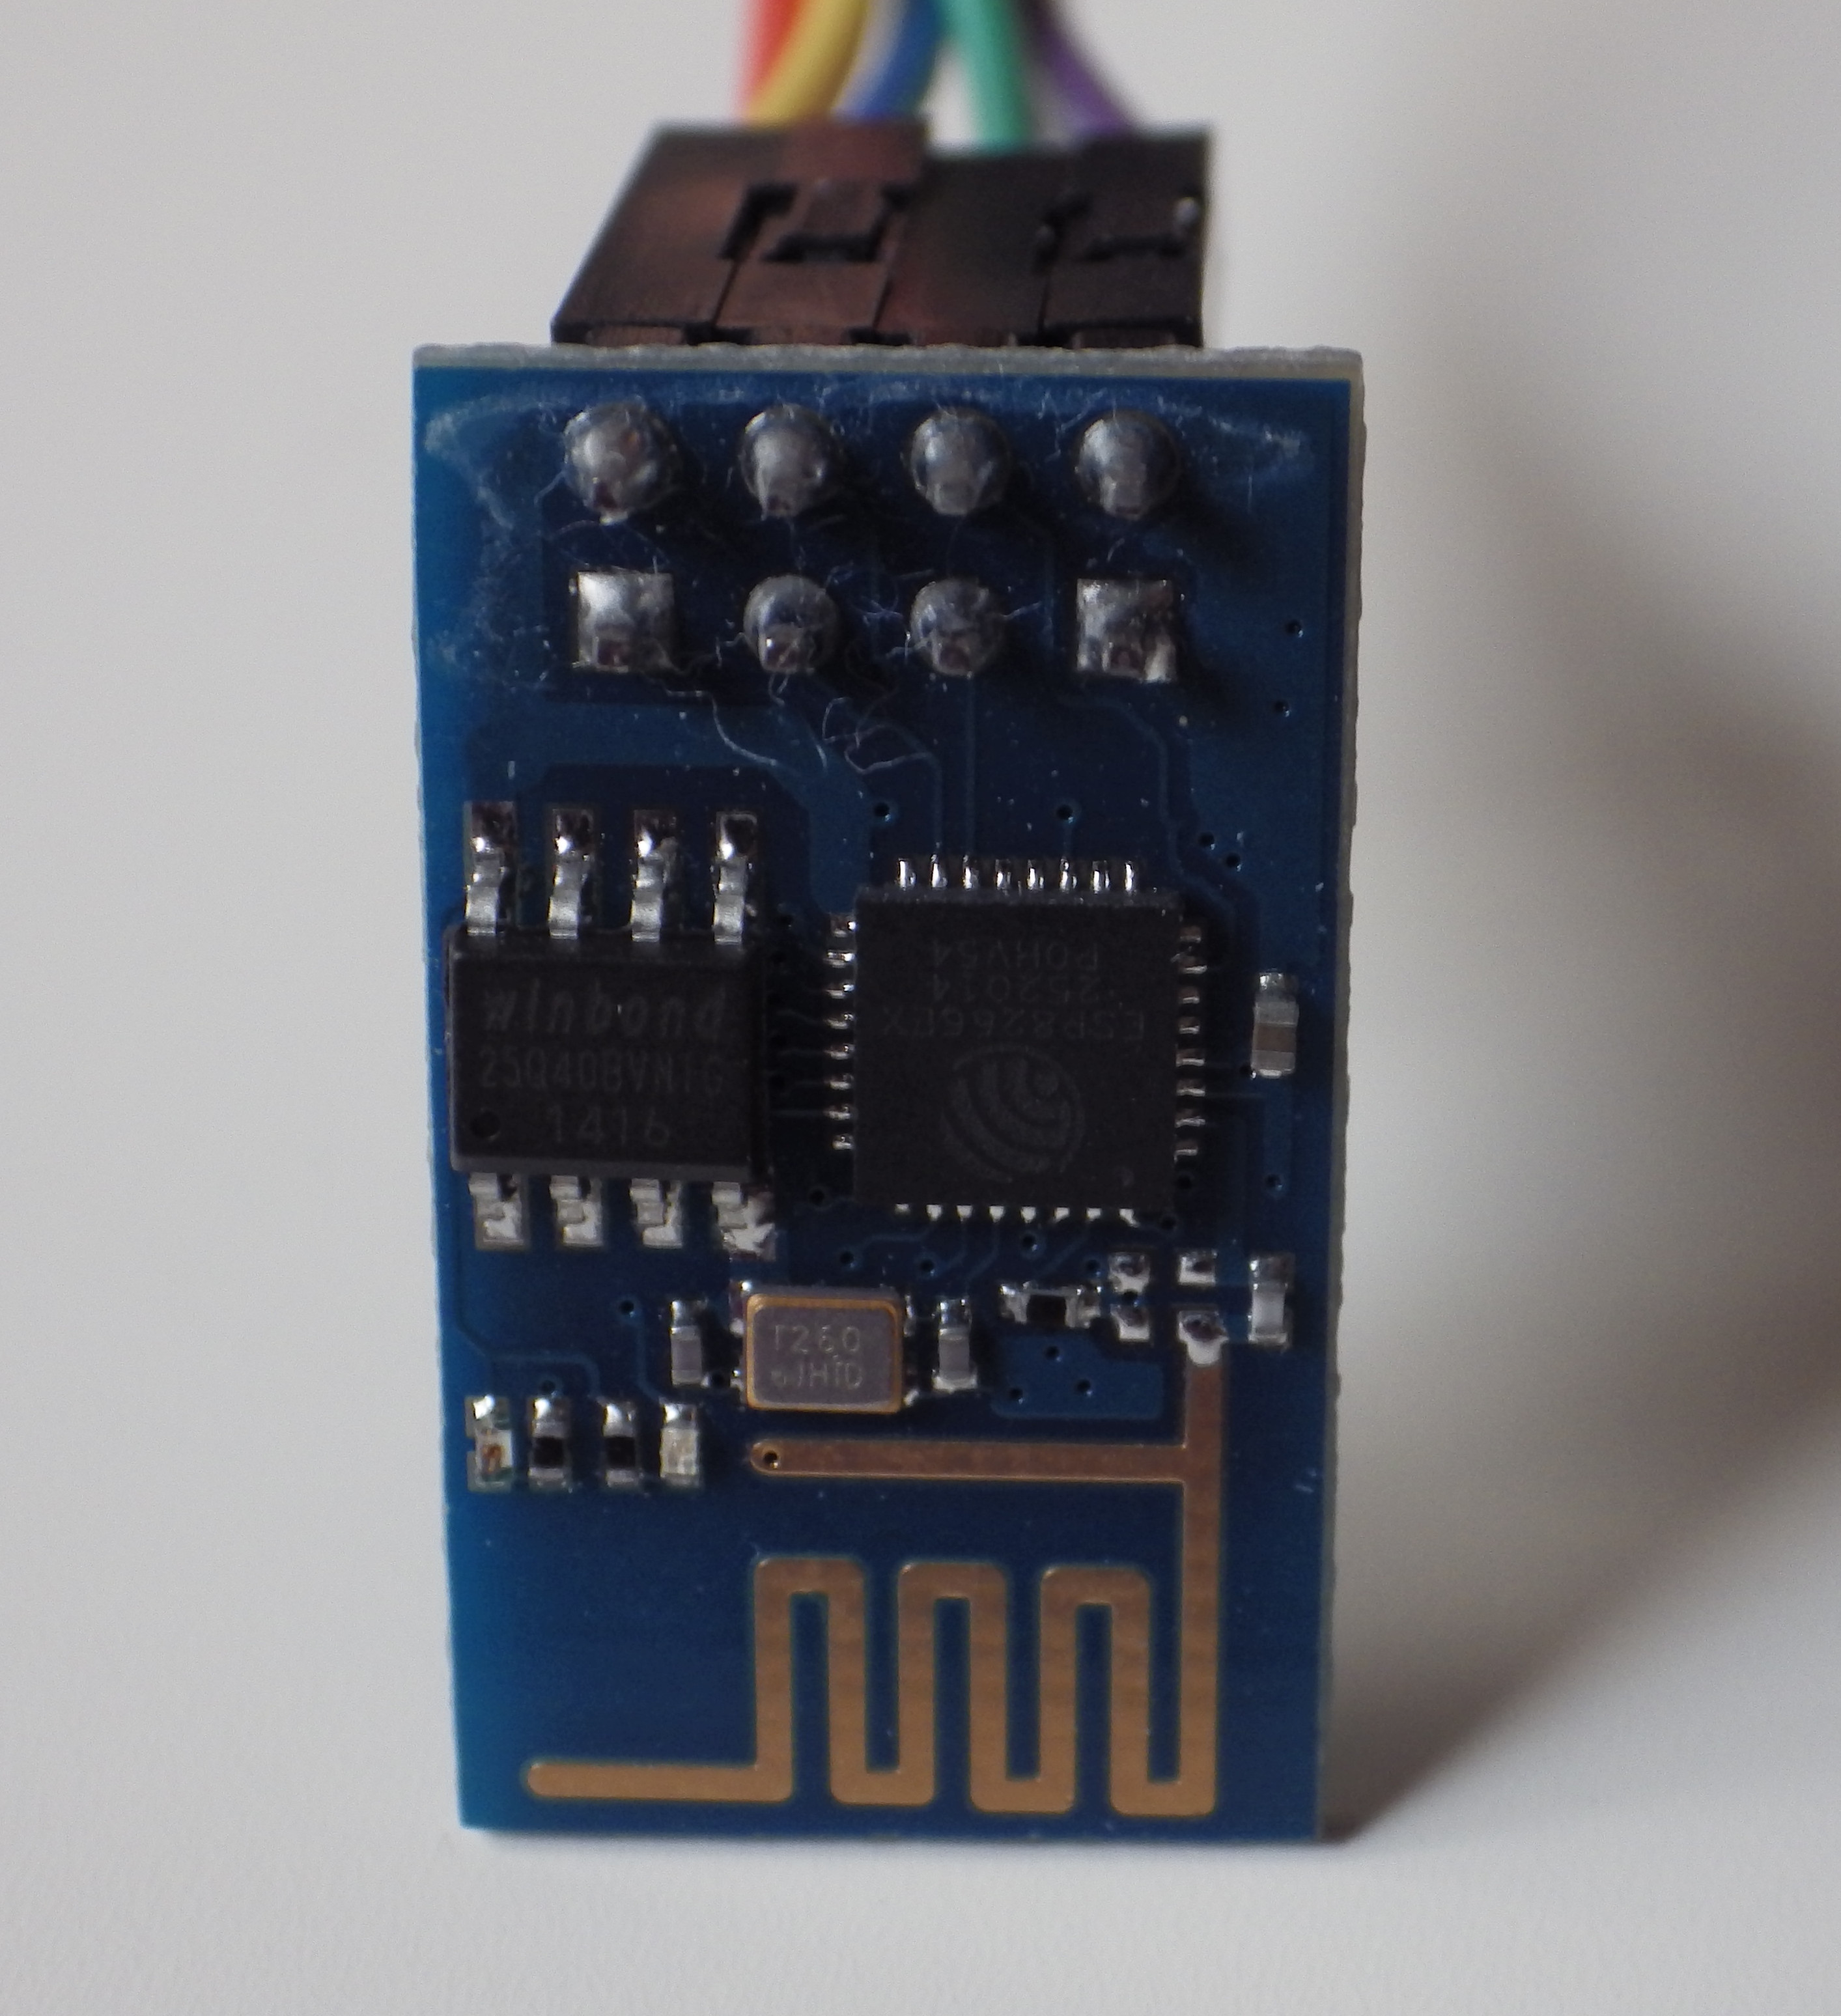
\includegraphics[height =60mm]{ESP8266.jpg}
	\label{ESP8266}
	\caption{Moduł WiFi ESP8266 zapewnia komunikację WiFi}
\end{figure}		

\subsubsection{Obudowa}
Obudowa projektu została zaprojektowana w programie Inventor oraz wydrukowana na drukarce 3D Pirx.
	\begin{figure}[!h]
	\centering
		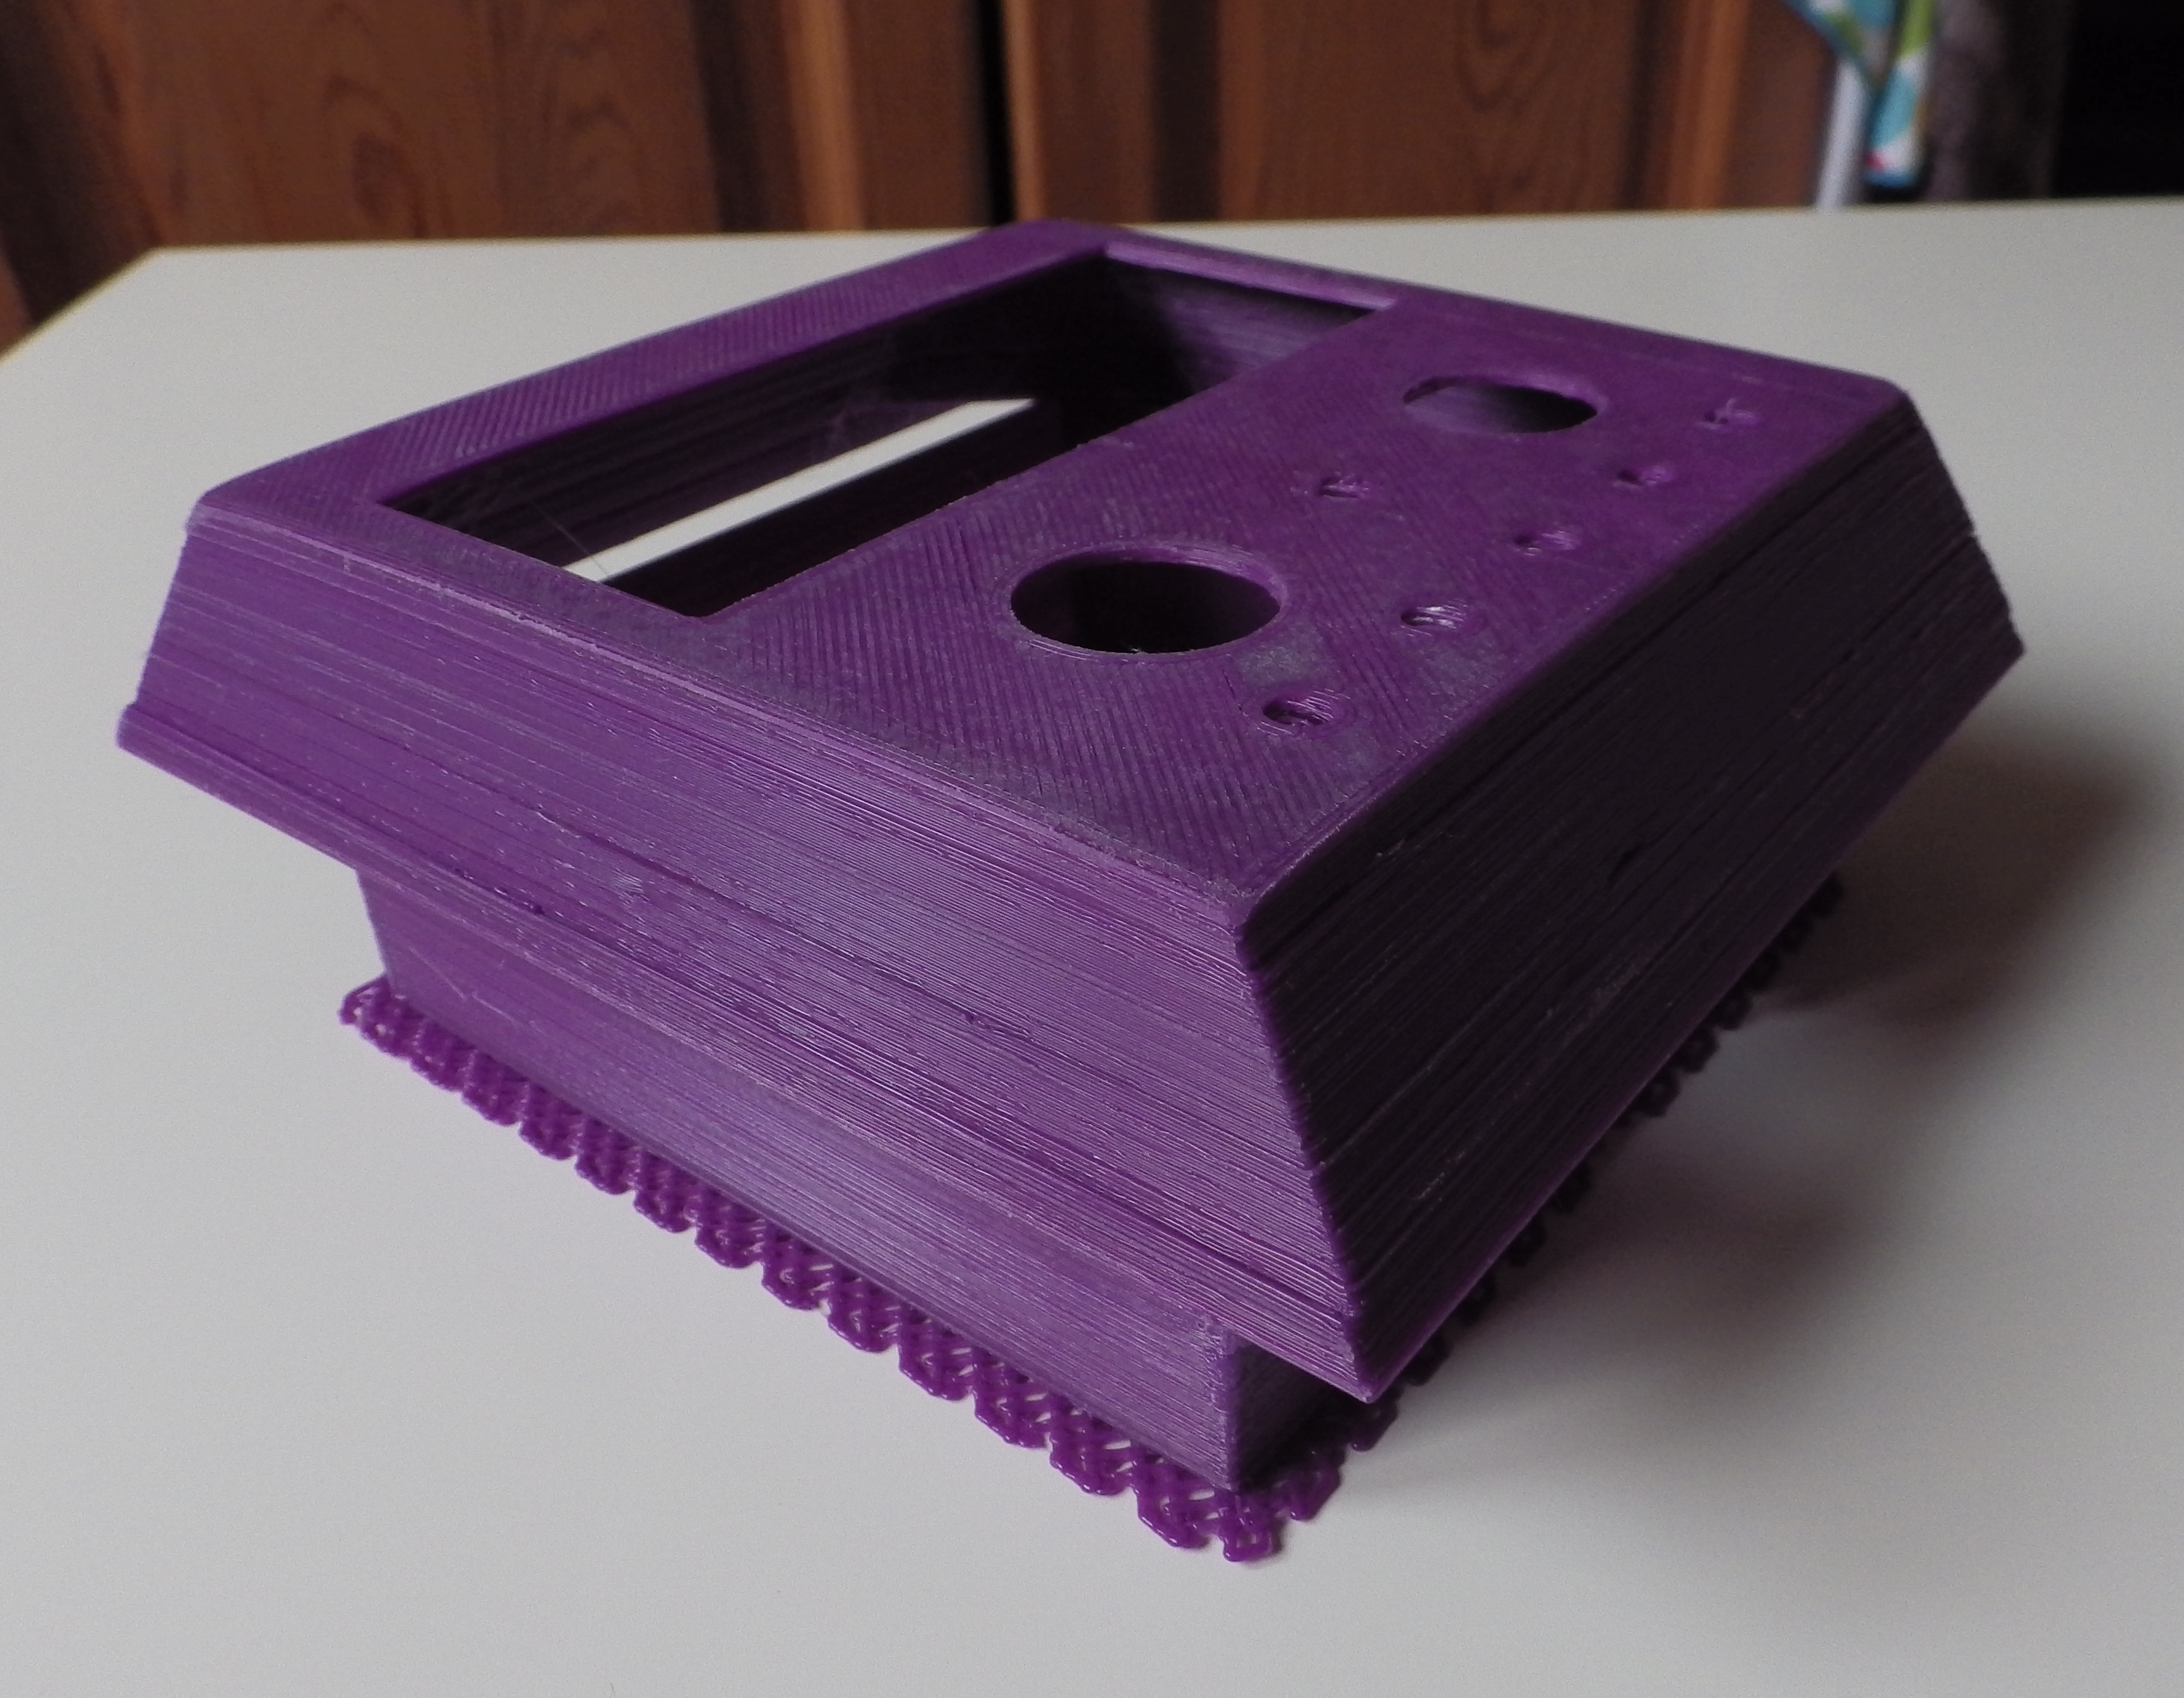
\includegraphics[height =60mm]{obudowa.jpg}
		\label{elktro}
		\caption{Obudowa projektu wydrukowana na drukarce 3D}
	\end{figure}

\newpage

\section{Koncepcja wprowadzenia rozwiązania w życie}
Nasze urządzenie jest bardzo rozbudowaną stacją pomiarową, która posiada aż 12 funkcjonalności:
\begin{itemize}
\item pomiar temperatury,
\item pomiar wilgotności względnej,
\item pomiar ciśnienia atmosferycznego,
\item pomiar poziomu oświetlenia,
\item pomiar stężenia dwutlenku węgla,
\item wykrywacz dymu i czadu,
\item alkomat,
\item wykrywacz wycieku gazu,
\item możliwość komunikacji zdalnej z urządzeniem mobilnym,
\item wizualizacja danych na wyświetlaczu LCD oraz w aplikacji mobilnej,
\item podświetlany wyświetlacz,
\item system akwizycji i wizualizacji danych.
\end{itemize}

Nasze rozwiązanie jest unikatowym połączeniem kilku współdziałających ze sobą czujników, które nie ma swoich odpowiedników na rynku. 

Projekt ma na celu naukę zachowań i zdrowych odruchów. Po dłuższym czasie korzystania z urządzenia użytkownik sam będzie wyczuwał co powinien zrobić, aby utrzymać odpowiedni mikroklimat. Grupą docelową tego projektu będą głównie szkoły, gdzie dzieci, poprzez kontakt z technologią będą spędzały czas w zdrowym środowisku, jednocześnie ucząc się jak je zachować.


\section{Możliwości dalszej rozbudowy}
W dalszej części naszego projektu pragniemy dodać więcej funkcjonalności w aplikacji mobilnej, takich jak trend zmiany temperatury, czy predykcję ciśnienia w ciągu najbliższych kilku godzin. Pozwoliłoby to nie tylko reagować na aktualne zagrożenia, ale również przewidywać i niwelować je już w zalążku.
Dodatkowo w przyszłości zostanie zaimplementowany system akwizycji danych na aplikację mobilną, dzięki któremu urządzenie będzie mogło uczyć się jakie błędy są popełniane najczęściej i ostrzegać przed nimi wcześniej.


\section{Podział prac w zespole}

W początkowym etapie pracy na projektem podzieliliśmy się zadaniami po równo, tak aby każdy z nas mógł wykazać się swoimi najlepszymi umiejętnościami oraz robił to, co lubi. I tak Jakub Szczepankiewicz podjął się zadania stworzenia aplikacji mobilnej, Jakub Porębski był odpowiedzialny za kalibrację czujników oraz za zaprojektowanie obudowy. Zadaniem Żanety było stworzenie obsługi czujników oraz komunikacji WiFi na FRDMKL25Z.

Jednakże nasza indywidualna praca nad projektem to nie wszystko. Są to również godziny spędzone na dyskusji, tysiące wiadomości wysyłanych do siebie oraz wiele pozytywnych emocji. W trakcie tworzenia projektu okazało się, że musimy wykorzystać wiedzę z bardzo wielu różnych dziedzin. Znajomość chemii ciała stałego pozwoliła skalibrować czujniki gazów. Projekt został napisany w wielu językach programowania, takich jak \mbox{MATLAB}, C i JAVA. Tylko dzięki współpracy i ciągłemu wspieraniu się wzajemnie udało nam się zbudować projekt, któremu każdy z osobna by nie podołał.
%Taki podział prac pozwolił nam na zorganizowany rozwój projektu. 

%\section{Zalecenia}
 % Opis rozwiązania zawierający:

%o   Szczegóły realizacji projektu – opis z uwzględnieniem wszystkich jego składowych (zarówno tych zaimplementowanych, jak tych, które wykraczają poza samą aplikację). Opis przygotujcie w formie tekstowej (maksymalnie 3000 znaków) oraz graficznej (obejmującej np. screeny aplikacji, schemat większego systemu itp.).

%o   Koncepcję wprowadzenia rozwiązania w życie – plan marketingowy (maksymalnie 2000 znaków).

%o   Możliwości dalszej rozbudowy (maksymalnie 1000 znaków).

%%o   Koncepcję podziału prac w zespole i zastosowane metody komunikacji (maksymalnie 1000 znaków).

%\section{ To już wysłaliśmy}
%\textbf{Ogólny opis projektu realizujący motto "Dom + technologia = lepsze życie" *
%Opis celów projektu i zarys planu na wprowadzenie go w życie (max 750 znaków)}

%Celem projektu jest zbudowanie systemu kontrolującego odpowiedni klimat w mieszkaniu. Urządzenie będzie monitorowało poziom stężenia CO2, wilgotność, temperaturę oraz natężenie światła i na podstawie zebranych będzie przekazywało wiadomość do użytkownika  na urządzenie mobilne o zalecanym przewietrzeniu pokoju, zakręceniu kaloryfera, czy zgaszeniu światła. System zostanie zbudowany w oparciu o moduł WiFi ESP8266 oraz czujniki zbudowane w technologii MEMS.

%\textbf{Opis innowacyjnych elementów projektu *
%Dlaczego projekt jest innowacyjny i co uczyni go unikalnym na rynku (max 500 znaków)}

%Dom jest najważniejszym środowiskiem, w jakim żyjemy. Dbamy o niego i staramy się, by panowała w nim „zdrowa” atmosfera. Nasze urządzenie pozwoli utrzymać odpowiedni mikroklimat w mieszkaniu, tak aby zatrzymać rozwój mikroorganizmów i zapewnić jak najmniejszy poziom zanieczyszczeń. Jednocześnie brak całkowitej kontroli nad ekosystemem mieszkania pozwoli nauczyć odpowiednich, zdrowych zachowań. 

\newpage

\end{document}